\documentclass[tikz,border=6pt]{standalone}
\usetikzlibrary{angles,quotes,calc,arrows.meta}

\begin{document}

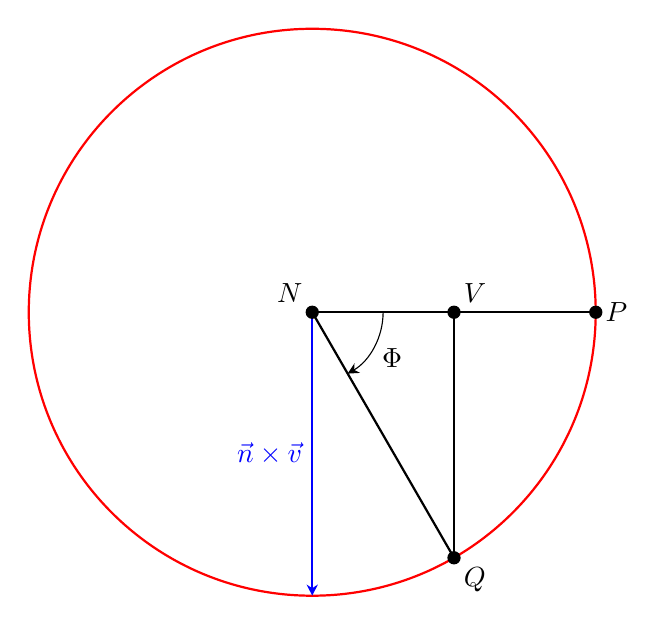
\begin{tikzpicture}[scale=1.2, 
  >={Stealth[length=4pt,width=4pt]},
  vector/.style={->,thick},
  charge/.style={circle,draw,fill=gray!20,minimum size=8pt,inner sep=0pt}
  ]

% Base point
\coordinate (N) at (0,0);
\coordinate (V) at (1.5,0);
% Circle
\def\R{3}
\draw[red, thick] (N) circle (\R);

% Points on circle
\def\alpha{0}
\def\beta{-60}
\coordinate (P) at ($(N)+({\R*cos(\alpha)}, {\R*sin(\alpha)})$);
\coordinate (Q) at ($(N)+({\R*cos(\beta)},  {\R*sin(\beta)})$);

%Lines
\draw[-, thick] (N) -- (P);
\draw[-, thick] (N) -- (Q);
\draw[-, thick] (V) -- (Q);

% Angle Phi
\pic[<-,draw,"$\Phi$",angle radius=9mm,angle eccentricity=1.3] {angle = Q--N--P};

% Downward vector
\draw[->, thick, blue] (N) -- ++(0,-\R) node[midway, left] {$\vec n \times \vec v$};

% Points
\fill (N) circle(2pt) node[above left] {$N$};
\fill (P) circle(2pt) node[right] {$P$};
\fill (Q) circle(2pt) node[below right] {$Q$};
\fill (V) circle(2pt) node[above right] {$V$};

\end{tikzpicture}

\end{document}